\documentclass[11pt]{article}
\usepackage{fontspec}
\setmainfont{NotoSerif-Regular.ttf}[Path=C:/Windows/Fonts/,ItalicFont=NotoSerif-Italic.ttf,BoldFont=NotoSerif-Bold.ttf,BoldItalicFont=NotoSerif-BoldItalic.ttf]
\usepackage[a4paper,margin=22mm]{geometry}
\usepackage{amsmath,amssymb,graphicx,xcolor,hyperref,needspace,tikz}
\usepackage[normalem]{ulem}
\let\MathUnderline\underline
\renewcommand{\underline}[1]{\ifmmode\MathUnderline{#1}\else\uline{#1}\fi}
\hypersetup{unicode=true,colorlinks=true,linkcolor=blue,pdfauthor={}}
\setlength{\parindent}{0pt}
\setlength{\parskip}{.4em}
\setlength{\emergencystretch}{3em}
\raggedright
\newcommand{\SourcePage}[2]{\par\smallskip\phantomsection\label{#1:source-page}{\small\sffamily\color{blue!55!black}#1}\par\smallskip}
\newcommand{\EvidenceBlock}[4]{%
 \par\smallskip\noindent\begin{minipage}{\linewidth}
 \begin{minipage}[t]{.47\linewidth}\vspace{0pt}\centering
 \csname evidence-#1-#2\endcsname\par
 {\scriptsize\SourceCropCaption\ #1}\par
 \end{minipage}\hfill
 \begin{minipage}[t]{.49\linewidth}\vspace{0pt}\raggedright
 {\small\color{orange!65!black}\textbf{#4} #3}\par
 \end{minipage}
 \end{minipage}\par\smallskip}
\newcommand{\Unclear}[3]{\EvidenceBlock{#1}{#2}{#3}{\ReadingCaption}}
\newcommand{\Incomplete}[3]{\EvidenceBlock{#1}{#2}{#3}{\IncompleteCaption}}
\newcommand{\SourceFigure}[3]{\EvidenceBlock{#1}{#2}{#3}{\DiagramCaption}}
\expandafter\def\csname evidence-GELFAND-P000001-module-letter\endcsname{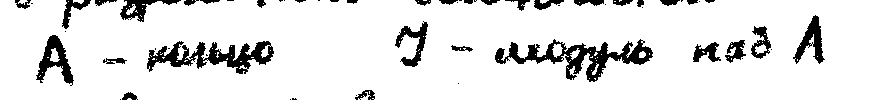
\includegraphics[width=\linewidth]{figures/gelfand-p000001-module-letter-original.png}}
\expandafter\def\csname evidence-GELFAND-P000001-diagram-blowup\endcsname{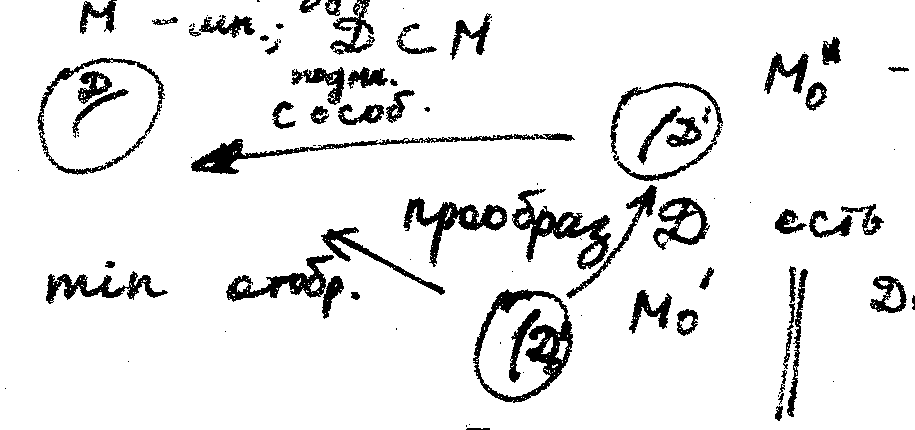
\includegraphics[width=\linewidth]{figures/gelfand-p000001-diagram-blowup-original.png}}
\expandafter\def\csname evidence-GELFAND-P000001-blowup-notation\endcsname{
\includegraphics[width=.43\linewidth]{figures/gelfand-p000001-upper-blowup-label-original.png}\hfill
\includegraphics[width=.50\linewidth]{figures/gelfand-p000001-lower-blowup-label-original.png}}
\expandafter\def\csname evidence-GELFAND-P000001-origin-example\endcsname{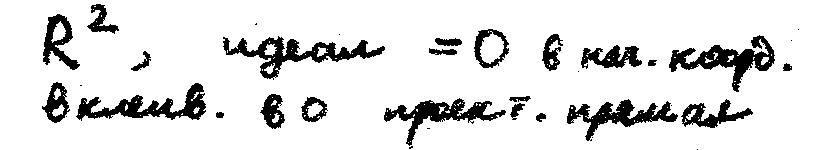
\includegraphics[width=\linewidth]{figures/gelfand-p000001-origin-example-original.png}}
\newcommand{\SourceCropCaption}{Оригинальные фрагменты:}\newcommand{\ReadingCaption}{Сомнительное чтение.}\newcommand{\IncompleteCaption}{Неразобранный фрагмент.}\newcommand{\DiagramCaption}{Рисунок и набранное описание.}
\hypersetup{pdftitle={Семинар И. М. Гельфанда — глава 1}}

\expandafter\def\csname evidence-GELFAND-P000002-ideal-selection\endcsname{
\includegraphics[width=\linewidth]{figures/gelfand-p000002-ideal-selection-part01-original-r1.png}}
\expandafter\def\csname evidence-GELFAND-P000002-open-set-notation\endcsname{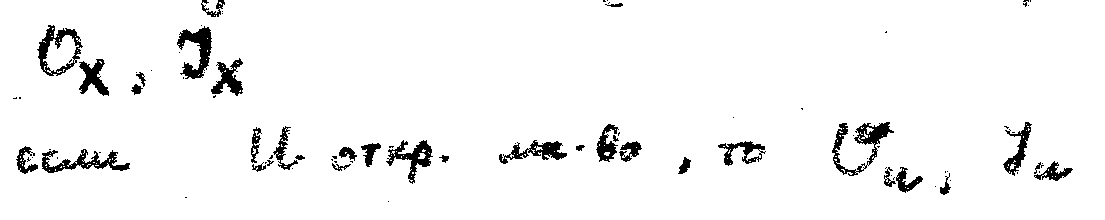
\includegraphics[width=\linewidth]{figures/gelfand-p000002-open-set-notation-part01-original-r2.png}}
\expandafter\def\csname evidence-GELFAND-P000002-fractions-sentence\endcsname{
\includegraphics[width=\linewidth]{figures/gelfand-p000002-fractions-sentence-part01-original-r1.png}\par\smallskip
\includegraphics[width=\linewidth]{figures/gelfand-p000002-fractions-sentence-part02-original-r1.png}\par\smallskip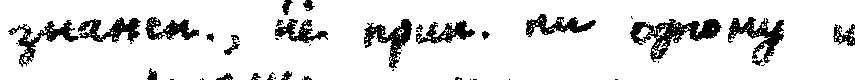
\includegraphics[width=\linewidth]{figures/gelfand-p000002-fractions-sentence-part03-original-r1.png}\par\smallskip
\includegraphics[width=\linewidth]{figures/gelfand-p000002-fractions-sentence-part04-original-r1.png}}
\expandafter\def\csname evidence-GELFAND-P000002-margin-grothendieck\endcsname{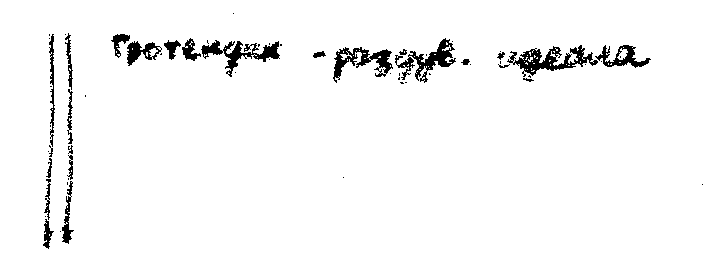
\includegraphics[width=\linewidth]{figures/gelfand-p000002-margin-grothendieck-part01-original-r1.png}}
\expandafter\def\csname evidence-GELFAND-P000002-quadratic-coefficients\endcsname{
\includegraphics[width=\linewidth]{figures/gelfand-p000002-quadratic-coefficients-part01-original-r1.png}}
\expandafter\def\csname evidence-GELFAND-P000002-last-sign\endcsname{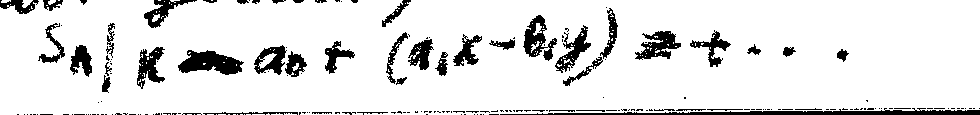
\includegraphics[width=\linewidth]{figures/gelfand-p000002-last-sign-part01-original-r1.png}}
\expandafter\def\csname evidence-GELFAND-P000003-directions\endcsname{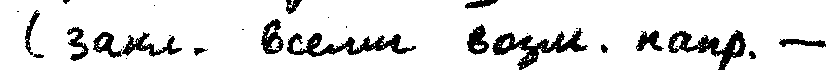
\includegraphics[width=\linewidth]{figures/gelfand-p000003-directions-part01-original-r1.png}\par\smallskip
\includegraphics[width=\linewidth]{figures/gelfand-p000003-directions-part02-original-r1.png}}
\expandafter\def\csname evidence-GELFAND-P000003-cross-cancellation\endcsname{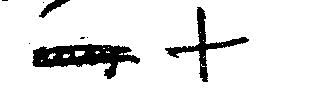
\includegraphics[width=\linewidth]{figures/gelfand-p000003-cross-cancellation-part01-original-r1.png}}
\expandafter\def\csname evidence-GELFAND-P000003-ising-cancellation\endcsname{
\includegraphics[width=\linewidth]{figures/gelfand-p000003-ising-cancellation-part01-original-r1.png}}
\expandafter\def\csname evidence-GELFAND-P000003-configuration-letter\endcsname{
\includegraphics[width=\linewidth]{figures/gelfand-p000003-configuration-letter-part01-original-r2.png}}
\expandafter\def\csname evidence-GELFAND-P000003-energy-cancellation\endcsname{
\includegraphics[width=\linewidth]{figures/gelfand-p000003-energy-cancellation-part01-original-r1.png}}
\expandafter\def\csname evidence-GELFAND-P000003-energy-case\endcsname{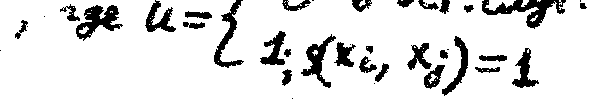
\includegraphics[width=\linewidth]{figures/gelfand-p000003-energy-case-part01-original-r2.png}\par\smallskip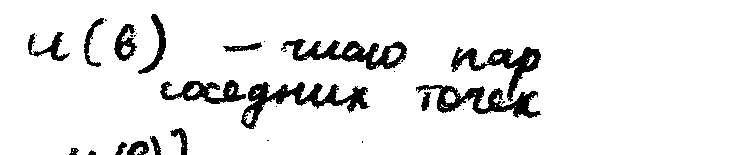
\includegraphics[width=\linewidth]{figures/gelfand-p000003-energy-case-part02-original-r3.png}}
\expandafter\def\csname evidence-GELFAND-P000003-partition-domain\endcsname{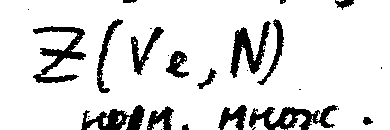
\includegraphics[width=\linewidth]{figures/gelfand-p000003-partition-domain-part01-original-r1.png}\par\smallskip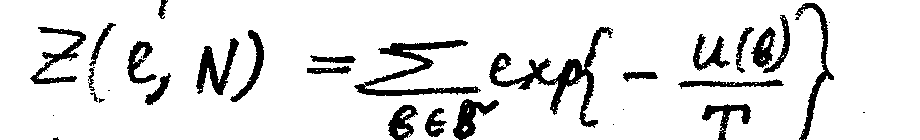
\includegraphics[width=\linewidth]{figures/gelfand-p000003-partition-domain-part02-original-r1.png}}
\expandafter\def\csname evidence-GELFAND-P000003-attraction-note\endcsname{
\includegraphics[width=\linewidth]{figures/gelfand-p000003-attraction-note-part01-original-r1.png}}
\expandafter\def\csname evidence-GELFAND-P000003-density-cancellation\endcsname{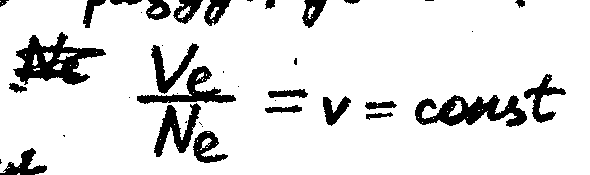
\includegraphics[width=\linewidth]{figures/gelfand-p000003-density-cancellation-part01-original-r1.png}}
\begin{document}
{\large\bfseries Семинар Гельфанда — глава 1}\par
{\small Начало читательского издания. Исходные страницы 1–3. Текст и формулы набраны; каждое сомнительное чтение сопровождается исходным фрагментом. Рабочий отрывок; полная глава готовится.}\par\medskip
\SourcePage{GELFAND-P000001}{unlabelled}
Понед. $21/\mathrm{IX}$.
Декартовы и булевы произв. групп.

«Хиронака: о разрешении особенностей».
\underline{Гельфанд}

$A$ — кольцо, $\mathcal{J}$ — модуль над $A$.
\Unclear{GELFAND-P000001}{module-letter}{Буква модуля и идеала передана как $\mathcal{J}$; возможны $\mathcal{I}$ или $J$.}

Раздутие — ?
$M$ — мн.; $D\subset M$.
[Под $D$:] подмн. с особ.

$M_0^H$ — раздутие. Blowing-up.
Прообраз $D$ есть $D'$ мн. разм. $n-1$.
$D_0$ — $(n-1)$-мерное.
\SourceFigure{GELFAND-P000001}{diagram-blowup}{Три обведённых рисунка: слева область с $D$, справа сверху область с $D'$ и подписью $M_0^H$, справа снизу область и подпись $M'_0$. Верхняя стрелка направлена влево; нижняя наклонная стрелка также влево, с подписью «непр. отобр.». Точные внутренние кривые, подписи и соединение нижней области с верхней требуют сравнения со сканом.}
\Unclear{GELFAND-P000001}{blowup-notation}{Верхний индекс у $M_0$ похож на $H$; подпись нижней области похожа на $M'_0$.}

Конструкция — Гротендик.
$A$ — кольцо, $\mathcal{J}$ — модуль.
\underline{Прим.} $A$ — кольцо ф-й;
$\mathcal{J}$ — идеал ф-й, обр. в $0$ на $D$.

Получится пучок колец и пучок модулей.
$A$ — кольцо, $\mathcal{J}$ — идеал.
Построим $X$, $O_X$ — пучок колец,
$\mathcal{J}_X$ — пучок идеалов, чтобы
\begin{gather*}
 (A,\mathcal{J})\ \longleftarrow\ (X,O_X,\mathcal{J}_X).
\end{gather*}
[Под стрелкой:] лин. отобр.

$(A,\mathcal{J})$ — пучок, порожд. $1$-м ид.

$\mathcal{J}_X$ обратим, т. е. идеал кольца:
$\exists f\in\mathcal{J}_X$ такого, что $O_Xf=\mathcal{J}_X$.
[Над формулой, стрелка к $\exists$:] образ.

(Идеал — главный, если $\mathcal{J}$ — идеал.)
Тогда многообр. нулей — $1$ ур-е.

$A$ — кольцо, $\mathcal{J}$ — идеал.
\underline{Тип. пример:} $R^2$, идеал $=0$ в нач. коорд.
\Unclear{GELFAND-P000001}{origin-example}{Следующая строка: «Вклеив. в $0$ проект. прямой»; начало может читаться «Оклеив.».}

$A$, $\mathcal{J}$ — мод.
\begin{gather*}
 \mathcal{J}\otimes_A\mathcal{J},\qquad
 \mathcal{J}\otimes_A\mathcal{J}\otimes_A\mathcal{J},\ldots
\end{gather*}
[Над группами тензорных произведений:] симм.; симм.

Рассм. форм. суммы
\begin{gather*}
 \sum_{k=0}^{N}a_kz^k.
\end{gather*}
Склад. и умн.
$x\otimes y=y\otimes x$.
\begin{gather*}
 a_0\in A,\qquad a_1\in\mathcal{J},\qquad
 a_2\in\mathcal{J}\otimes_A\mathcal{J}\quad\text{—}
\end{gather*}

\SourcePage{GELFAND-P000002}{unlabelled}
Кольцо таких сумм $S_A(\mathcal{J})$.
Рассм. однор. идеалы
[над строкой вставлено:] (градуир.).
(Вместе с многочленом сод. все его однородные.)

Рассм. все простые однор. идеалы в $S_A(\mathcal{J})$.
Выбр. идеалы, к-рые сод. все мн., нач. с $1$-й степени.
\Unclear{GELFAND-P000002}{ideal-selection}{Конец строки после «сод. все» лучше читается как «мн., нач. с $1$-й степени»; средние штрихи сокращения «нач.» остаются не вполне различимыми.}

Совок. идеалов $X$. (Топология Зарисского.)
$O_X$, $\mathcal{J}_X$.
Если $U$ откр. мн-во, то $O_U$, $\mathcal{J}_U$.
\Unclear{GELFAND-P000002}{open-set-notation}{После «то» первая буква совпадает по форме с $O_X$ выше, вторая — с буквой идеала: $O_U$, $\mathcal{J}_U$; последняя может быть $\mathcal{I}_U$.}

$S_A(\mathcal{J})$ — всё кольцо.
Кольцо отношений, числ., знамен., не прин. ни одному из идеалов.
Локализ. кольцо на это мн-во.
Отнош. $1$-й степени $\mathcal{J}_U$.
\Unclear{GELFAND-P000002}{fractions-sentence}{В строке об отношениях не вполне ясны сокращения «числ.-знамен.» и то, относится ли «не прин.» только к знаменателю. Слова не дополнены по смыслу.}
[Справа, две стрелки вниз:] Гротендик — раздуть идеально.
\Unclear{GELFAND-P000002}{margin-grothendieck}{Правая помета читается как «Гротендик — раздуть идеально»; последнее слово возможно «идеально» или «идеалы».}

$A$ — кольцо многочл. $2$-х пер.
$\mathcal{J}$ — идеал из мн. $P(0,0)=0$.
\begin{gather*}
 A=\{P(x,y)\},\qquad
 \mathcal{J}=P(x,y)=a_1x+b_1y+\cdots .
\end{gather*}
\begin{gather*}
 \mathcal{J}\otimes_A\mathcal{J}\ \longleftrightarrow
 \{a_2x^2+2b_2xy+cy^2+\cdots\}.
\end{gather*}
\Unclear{GELFAND-P000002}{quadratic-coefficients}{Коэффициенты в квадратном многочлене читаются $a_2$, $2b_2$, $c$; индекс у $c$ и вид толстой двусторонней стрелки не уверены.}

Из-за переброски получ. то же, что квадрат идеала.
Тогда — идеал из мн., равных $0$ в этой точке.
Во что она раздуется? ?

\begin{gather*}
 \sum P_k(x,y)z^k,\qquad P_k(x,y)=ax^k+\cdots .
\end{gather*}
[Справа:] Градуир. $\Sigma$ тенз. произвед.
\begin{gather*}
 A=\{P_0(x,y)\}\longrightarrow S_A(\mathcal{J}),\qquad
 P_0(x,y)\sim P_0(x,y).
\end{gather*}
Набор простых идеалов, получ. из ид. $P(0,0)=0$.
\begin{gather*}
 S_A\sim\sum P_kz^k,\qquad P_k\in\mathcal{J}^k,\qquad
 K\sim\sum P_kz^k.
\end{gather*}
Дост. найти max ид. факторкольца —
(чтобы найти ид., сод. данный).
\begin{gather*}
 S_A/K\ \longleftrightarrow\ a_0+(a_1x-b_1y)z+\cdots .
\end{gather*}
\Unclear{GELFAND-P000002}{last-sign}{В последней формуле перед $b_1y$ виден минус, хотя на следующем скане стоит плюс. Сохранён видимый минус; направление толстой стрелки также не вполне ясно.}

\SourcePage{GELFAND-P000003}{2}
Все однор. max ид. в нём и будут точками расширения.
Своб. члена нет (тогда и $1$).
\begin{gather*}
 (a_1x+b_1y)z.
\end{gather*}
Только $1$ лин. комб. $x$ и $y$.
($2$ нет, т. к. тогда все.)

Идеалы опр. напр. на плоскости
(замк. всеми возм. напр. — $\sigma$-процесс).
\Unclear{GELFAND-P000003}{directions}{Сокращения в скобках читаются «замк. всеми возм. напр.»; первое слово и значение знака $\sigma$ не утверждаются.}
\Needspace{48mm}\underline{Задача.} В пр-ве
[зачёркнуто:] \Unclear{GELFAND-P000003}{cross-cancellation}{Зачёркнутое слово перед рисунком не читается.}
\par\smallskip\noindent\begin{minipage}{\linewidth}\begin{minipage}[t]{.47\linewidth}\centering\vspace{0pt}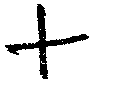
\includegraphics[width=30mm]{figures/gelfand-p000003-cross-diagram-original-r1.png}\par{\scriptsize Исходный рисунок}\end{minipage}\hfill\begin{minipage}[t]{.49\linewidth}\centering\vspace{0pt}\begin{tikzpicture}[scale=0.5]
 \draw (-0.8,0)--(0.8,0);
 \draw (0,-0.7)--(0,0.8);
\end{tikzpicture}\par{\scriptsize Наборное воспроизведение}\end{minipage}\end{minipage}\par\smallskip
Что получ. при заклеивании?
\begin{gather*}
 z=0,\qquad xy=0,\qquad \mathcal{J}=(z,xy).
\end{gather*}
[Под системой проведена черта.]

\underline{Добрушин.}
[Зачёркнуто перед «Найти»:] \Unclear{GELFAND-P000003}{ising-cancellation}{Зачёркнутое начало строки не читается уверенно.}
Найти пример газа, в к-ром сущ. фаз. переходы.
Куб целочисл. решётки.
$\ell$ — длина. $V_\ell=\ell^\nu$.
$N$ точ. $N<V_\ell$.
Могут заним. полож. на решётке
$\theta=(x_1,\ldots,x_N)$.
\Unclear{GELFAND-P000003}{configuration-letter}{Знак конфигурации передан как $\theta$; рукописный знак также похож на $b$ или кириллическое «в».}

Модель Изинга.
[Перед формулой густой зачёркнутый знак:]
\Unclear{GELFAND-P000003}{energy-cancellation}{Отдельный зачёркнутый знак перед $U(\theta)$ не читается.}
\begin{gather*}
 U(\theta)=-\frac12\sum_{i\ne j}u(x_i,x_j),\qquad
 u=\begin{cases}
 0&\text{в ост. случ.},\\
 1;&\rho(x_i,x_j)=1.
 \end{cases}
\end{gather*}
$u(\theta)$ — число пар соседних точек.
\Unclear{GELFAND-P000003}{energy-case}{В условии второй ветви виден знак, похожий на $\rho$; точка с запятой после $1$ сохранена. В подписи ниже первая буква похожа на малое $u$, а не $U$.}

Осн. аксиом — распр. Гиббса.
\begin{gather*}
 \mathsf{P}(B)=
 \frac{\displaystyle\sum_{\theta\in B}\exp\{-U(\theta)/T\}}
 {Z(V_\ell,N)},\qquad T>0\text{ — темпер.}
\end{gather*}
[Под знаменателем:] норм. множ.
\begin{gather*}
 Z(\ell,N)=\sum_{\theta\in\mathcal{B}}\exp\{-U(\theta)/T\}.
\end{gather*}
\Unclear{GELFAND-P000003}{partition-domain}{В знаменателе первой формулы написано $Z(V_\ell,N)$, следующая строка — $Z(\ell,N)$; знак множества под суммой похож на $\mathcal{B}$. Не исправлено по согласованности.}

Молекулы притяг.
([Два закрашенных знака со стрелками:] соседи $>$ их вероятн.)
\Unclear{GELFAND-P000003}{attraction-note}{В скобках после «Молекулы притяг.» закрашенные знаки и стрелки; чтение «соседи $>$ их вероятн.» не уверено.}
$B\subset\mathcal{B}$ — совок. распол.
\begin{gather*}
 p(\theta)=\frac{\exp\{-U(\theta)/T\}}{Z(\ell,N)}.
\end{gather*}
Пред. перех. $\ell\to\infty$, куб раздув. до $\infty$.
$N_\ell$ зав. от $\ell$.
[Зачёркнутый знак перед дробью:]
\Unclear{GELFAND-P000003}{density-cancellation}{Зачёркнутый знак перед $V_\ell/N_\ell$ не читается.}
\begin{gather*}
 \frac{V_\ell}{N_\ell}=v=\mathrm{const}.
\end{gather*}
Реш. увеличивается.
Можно показ., что
\begin{gather*}
 \frac1{N_\ell}\log Z(\ell,N_\ell)\longrightarrow f(v,T).
\end{gather*}
\clearpage\section*{Полные примечания к чтениям}
\subsection*{GELFAND-0001-U001}
\EvidenceBlock{GELFAND-P000001}{module-letter}{После A — кольцо стоит рукописная буква с развилкой сверху и нижним крюком; она повторяется у модуля и идеала.}{Наблюдение.}
\par\smallskip\noindent\textbf{Варианты: } \(\mathcal{J}\); \(\mathcal{I}\); J\par
\par\smallskip\noindent\textbf{Историческая помета: } В тексте использован каллиграфический J как графический кандидат; обозначение не определено по математическому смыслу.\par
\par\smallskip\noindent\textbf{Повторное сравнение: } В трёх отдельных вхождениях при 5×/10× видны развилка сверху и нижний крюк. Это подтверждает единое графическое обозначение,но не устанавливает однозначно условное различие I/J.\par
\subsection*{GELFAND-0001-U002}
\EvidenceBlock{GELFAND-P000001}{diagram-blowup}{В верхней половине три округлых контура с внутренними кривыми, две стрелки влево; над ними и рядом D, D', M и индексы.}{Наблюдение.}
\par\smallskip\noindent\textbf{Варианты: } Не предложены.\par
\par\smallskip\noindent\textbf{Историческая помета: } Неуверенные внутренние кривые и соединения не перерисованы. Описание и описание исходного рисунка сохраняют источник для проверки.\par
\par\smallskip\noindent\textbf{Повторное сравнение: } Полная вырезка рисунка теперь показана при его набранном описании. Видны оба наконечника стрелок влево. От нижнего контура вверх к области около D идёт отдельный изогнутый штрих; его точное соединение с верхним контуром не утверждается.\par
\subsection*{GELFAND-0001-U003}
\EvidenceBlock{GELFAND-P000001}{blowup-notation}{Верхний индекс у \(M_0\) выглядит как H; у нижней области над \(M_0\) стоит короткий штрих.}{Наблюдение.}
\par\smallskip\noindent\textbf{Варианты: } \(M_0^H\); \(M'_0\); \(M_0^N\); \(M'_0\)\par
\par\smallskip\noindent\textbf{Историческая помета: } Индексы и штрих требуют сравнения с оригиналом.\par
\par\smallskip\noindent\textbf{Повторное сравнение: } Непосредственно при чтении помещены отдельные крупные вырезки тёмного верхнего индекса и нижнего штриха. Нижний штрих различим; для тёмного верхнего знака нет достаточного основания исключить N в пользу H.\par
\subsection*{GELFAND-0001-U006}
\EvidenceBlock{GELFAND-P000001}{origin-example}{Справа от примера \(R^2\) строка начинается связной группой букв и оканчивается в 0 проект. прямой.}{Наблюдение.}
\par\smallskip\noindent\textbf{Варианты: } Вклеив. в 0 проект. прямой; Оклеив. в 0 проект. прямой\par
\par\smallskip\noindent\textbf{Историческая помета: } Фраза дана внутри пометы сомнительного чтения, без выбора по смыслу раздутия.\par
\par\smallskip\noindent\textbf{Повторное сравнение: } Широкий контекст и детали 5×/10× существенно поддерживают начальную В и сокращение «Вклеив.». Исторический вариант сохранён; формулировка не заменена стандартным определением раздутия.\par

\subsection*{GELFAND-0001-U007}
\EvidenceBlock{GELFAND-P000002}{ideal-selection}{Повторное чтение увеличенного исходного фрагмента лучше даёт мн., нач. с 1-й степени; средние штрихи сокращения нач. всё ещё не полностью различимы.}{Наблюдение.}
\par\smallskip\noindent\textbf{Кандидаты: } мн., нач. с 1-й степени; мн., к-ст. с 1-й степенью\par
\par\smallskip\noindent\textbf{Прежнее примечание: } Первый кандидат выбран по графике исходной строки; он не заменён стандартным определением Proj.\par
\par\smallskip\noindent\textbf{Новое сравнение с источником: } В полной строке и отдельных деталях 5×/10× видны конец строки и начальное «Выбр.». Раскрытие последнего как выбора либо исключения не устанавливается из конструкции. В английском тексте сокращение сохранено. В конце графика лучше поддерживает «нач.»; прежняя альтернатива сохранена.\par

\subsection*{GELFAND-0001-U008}
\EvidenceBlock{GELFAND-P000002}{open-set-notation}{При отдельном повторном просмотре первая буква после то совпадает по форме с \(O_X\) выше; вторая совпадает с буквой идеала с нижним крюком.}{Наблюдение.}
\par\smallskip\noindent\textbf{Кандидаты: } \(O_U,J_U\); \(O_U,I_U\)\par
\par\smallskip\noindent\textbf{Прежнее примечание: } Первоначальное чтение первой буквы как J исправлено по скану. Возможное различие I/J второй буквы остаётся, независимо от стандартной конструкции пучка.\par
\par\smallskip\noindent\textbf{Новое сравнение с источником: } Исправленный общий фрагмент включает нижние индексы полностью. Округлая первая буква и вторая с развилкой и нижним крюком совпадают с парой выше. Это поддерживает O и букву идеала, но не устраняет условного различия I/J. Отдельные детали просмотрены при 5×/10×.\par

\subsection*{GELFAND-0001-U009}
\EvidenceBlock{GELFAND-P000002}{fractions-sentence}{После Кольцо отношений видны числ., знамен., не прин. ни одному из идеалов, но границы сокращений и область действия последней фразы не ясны.}{Наблюдение.}
\par\smallskip\noindent\textbf{Кандидаты: } числ., знамен., не прин. ни одному из идеалов; числ.; знамен. не прин. ни одному из идеалов\par
\par\smallskip\noindent\textbf{Прежнее примечание: } Пунктуация не исправлена определением локализации.\par
\par\smallskip\noindent\textbf{Новое сравнение с источником: } Четыре перекрывающихся фрагмента сохраняют конец «числ.», следующее «знамен.» и фразу об идеалах. Сокращения видны при 5×/10×, но пунктуация не устанавливает область ограничения. Недостающее уточнение не добавлено.\par

\subsection*{GELFAND-0001-U010}
\EvidenceBlock{GELFAND-P000002}{margin-grothendieck}{Правая помета у двух вертикальных стрелок: Гротендик — раздуть ...; последнее слово написано связно.}{Наблюдение.}
\par\smallskip\noindent\textbf{Кандидаты: } идеально; идеалы\par
\par\smallskip\noindent\textbf{Прежнее примечание: } Последнее слово не утверждается.\par
\par\smallskip\noindent\textbf{Новое сравнение с источником: } Общий фрагмент содержит обе стрелки вниз и всю помету. Конечные связные штрихи скорее дают «идеально», но не исключают «идеалы». Сохранены буквальный кандидат и альтернатива; фраза не превращена в определение.\par

\subsection*{GELFAND-0001-U011}
\EvidenceBlock{GELFAND-P000002}{quadratic-coefficients}{После J тензор J толстая двусторонняя отметка и квадратный многочлен; коэффициенты похожи на \(a_2\), \(2b_2\), c.}{Наблюдение.}
\par\smallskip\noindent\textbf{Кандидаты: } \(a_2x^2+2b_2xy+cy^2+\cdots\); \(a_2x^2+2b_2xy+c_2y^2+\cdots\)\par
\par\smallskip\noindent\textbf{Прежнее примечание: } Индекс последнего коэффициента и направление толстой отметки не уверены.\par
\par\smallskip\noindent\textbf{Новое сравнение с источником: } В полном контексте и деталях видны \(a_2\) и \(2b_2\). У c-образной буквы есть малый верхний штрих, который не даёт уверенного нижнего индекса 2. Толстая связь оставлена графическим кандидатом без утверждения изоморфизма.\par

\subsection*{GELFAND-0001-U012}
\EvidenceBlock{GELFAND-P000002}{last-sign}{У нижней границы \(a_0+(a_1x-b_1y)z+\cdots\); горизонтальный знак перед \(b_1y\) выглядит как минус.}{Наблюдение.}
\par\smallskip\noindent\textbf{Кандидаты: } \(a_0+(a_1x-b_1y)z+\cdots\); \(a_0+(a_1x+b_1y)z+\cdots\)\par
\par\smallskip\noindent\textbf{Прежнее примечание: } В теле сохранён видимый минус; следующий скан имеет плюс. Стрелка слева густо написана.\par
\par\smallskip\noindent\textbf{Новое сравнение с источником: } В увеличении знак перед \(b_1y\) горизонтален; пересекающего вертикального штриха не видно. На следующей странице стоит плюс. Обе записи сохранены; возможная математическая смена знака не исправляет текст. Направление толстой стрелки остаётся сомнительным.\par

\subsection*{GELFAND-0001-U013}
\EvidenceBlock{GELFAND-P000003}{directions}{В скобках после плоскости написано сокращение замк. всеми возм. напр. — знак, похожий на сигму, процесс.}{Наблюдение.}
\par\smallskip\noindent\textbf{Кандидаты: } замк. всеми возм. напр. — σ-процесс; зам. всеми возм. напр. — σ-процесс\par
\par\smallskip\noindent\textbf{Прежнее примечание: } Сокращения не раскрыты и не заменены термином по смыслу.\par
\par\smallskip\noindent\textbf{Новое сравнение с источником: } Начальное сокращение и сигма-подобный знак просмотрены при 5×/10×. Последний короткий штрих сокращения не вполне надёжен. В переводе соседние ясные сокращения раскрыты, а «замк.» оставлено явно нераскрытым.\par

\subsection*{GELFAND-0001-U014}
\EvidenceBlock{GELFAND-P000003}{cross-cancellation}{Между В пр-ве и крестом густо зачёркнута короткая группа букв.}{Наблюдение.}
\par\smallskip\noindent\textbf{Кандидаты: } Кандидаты не предложены.\par
\par\smallskip\noindent\textbf{Прежнее примечание: } Само зачёркивание отмечено; текст под ним нельзя прочитать уверенно.\par
\par\smallskip\noindent\textbf{Новое сравнение с источником: } Плотное горизонтальное зачёркивание не читается и при 10×. Отдельный исходный крест показан рядом с имеющимся двухштриховым наборным воспроизведением. Утолщённые концы не устанавливают намеренных стрелок; оставлены две пересекающиеся линии без наконечников.\par

\subsection*{GELFAND-0001-U016}
\EvidenceBlock{GELFAND-P000003}{ising-cancellation}{Под именем Добрушин перед Найти полностью зачёркнута группа букв.}{Наблюдение.}
\par\smallskip\noindent\textbf{Кандидаты: } Кандидаты не предложены.\par
\par\smallskip\noindent\textbf{Прежнее примечание: } Видимая отмена сохранена, исходное слово не реконструировано.\par
\par\smallskip\noindent\textbf{Новое сравнение с источником: } Общий контекст устанавливает место перед «Найти»; при 5×/10× видны плотные пересекающиеся штрихи. Полного слова они не дают, поэтому кандидат не выдуман.\par

\subsection*{GELFAND-0001-U017}
\EvidenceBlock{GELFAND-P000003}{configuration-letter}{Перед \((x_1,\ldots,x_N)\) и далее в формулах знак с округлой нижней частью и тёмным верхним штрихом.}{Наблюдение.}
\par\smallskip\noindent\textbf{Кандидаты: } \(\theta\); \(b\); в\par
\par\smallskip\noindent\textbf{Прежнее примечание: } Во фрагменте применён θ как единый графический кандидат для этого повторяющегося знака.\par
\par\smallskip\noindent\textbf{Новое сравнение с источником: } Исправленный фрагмент включает знак слева и равенство целиком. Два вхождения просмотрены при 5×/10×. Разделённая петля и густой верхний штрих повторяются, но b либо кириллическая «в» надёжно не исключены. Чтение θ остаётся явно условным.\par

\subsection*{GELFAND-0001-U018}
\EvidenceBlock{GELFAND-P000003}{energy-cancellation}{Между Модель Изинга и \(U(\theta)\) находится отдельный полностью закрашенный знак.}{Наблюдение.}
\par\smallskip\noindent\textbf{Кандидаты: } Кандидаты не предложены.\par
\par\smallskip\noindent\textbf{Прежнее примечание: } Зачёркнутый знак не принят за математический оператор.\par
\par\smallskip\noindent\textbf{Новое сравнение с источником: } Знак остаётся непрозрачным при 5×/10×; тёмная масса и остатки штрихов не определяют оператор или букву. Сохранены место и зачёркивание без приписывания математической роли.\par

\subsection*{GELFAND-0001-U019}
\EvidenceBlock{GELFAND-P000003}{energy-case}{Во второй ветви u=... перед \((x_i,x_j)=1\) знак похож на ρ; ниже подпись начинается \(u(\theta)\).}{Наблюдение.}
\par\smallskip\noindent\textbf{Кандидаты: } \(\rho(x_i,x_j)=1\); \(\chi(x_i,x_j)=1\)\par
\par\smallskip\noindent\textbf{Прежнее примечание: } Виден знак после единицы, похожий на точку с запятой. Малое u в подписи не заменено на U.\par
\par\smallskip\noindent\textbf{Новое сравнение с источником: } Исправленный контекст содержит равенство целиком, а исправленная деталь 5×/10× — сам ρ-подобный знак. Прежняя узкая деталь не охватывала его и не считается свидетельством его чтения. Полная нижняя подпись начинается малой u-образной буквой. Пунктуация ветви и различие U/u сохранены; математический смысл обсуждается отдельно.\par

\subsection*{GELFAND-0001-U020}
\EvidenceBlock{GELFAND-P000003}{partition-domain}{Первая нормирующая величина выглядит \(Z(V_\ell,N)\), ниже написано \(Z(\ell,N)\); множество под второй суммой имеет форму рукописного B.}{Наблюдение.}
\par\smallskip\noindent\textbf{Кандидаты: } \(Z(V_\ell,N);\ Z(\ell,N);\ \theta\in B\); \(Z(V_\ell,N);\ Z(\ell,N);\ \theta\in\mathcal B\)\par
\par\smallskip\noindent\textbf{Прежнее примечание: } Различие аргументов сохранено. Символ множества не объявлен тождественным событию B по смыслу.\par
\par\smallskip\noindent\textbf{Новое сравнение с источником: } Отдельные детали 5×/10× подтверждают \(V_\ell\) в первом знаменателе и ell в следующей строке. У множества под второй суммой есть верхний дополнительный штрих, поддерживающий отдельный графический кандидат; обычное и каллиграфическое B всё ещё различаются неуверенно. Кандидаты события и множества конфигураций не отождествлены.\par

\subsection*{GELFAND-0001-U021}
\EvidenceBlock{GELFAND-P000003}{attraction-note}{После Молекулы притяг. скобки с закрашенными знаками, стрелками и словами соседи, вероятн.}{Наблюдение.}
\par\smallskip\noindent\textbf{Кандидаты: } соседи > их вероятн.; соседи > его вероятн.\par
\par\smallskip\noindent\textbf{Прежнее примечание: } Условная подпись передана только как кандидат, рисунок не превращён в точное утверждение.\par
\par\smallskip\noindent\textbf{Новое сравнение с источником: } Закрашенные знаки, стрелки и подпись показаны вместе. При 5×/10× местоимение ближе к «его», чем к «их», но неполная фраза не даёт точного утверждения. Унаследованный кандидат в тексте оставлен явно сомнительным; обе прежние альтернативы сохранены.\par

\subsection*{GELFAND-0001-U022}
\EvidenceBlock{GELFAND-P000003}{density-cancellation}{Перед \(V_\ell/N_\ell\) густо зачёркнута короткая отметка.}{Наблюдение.}
\par\smallskip\noindent\textbf{Кандидаты: } Кандидаты не предложены.\par
\par\smallskip\noindent\textbf{Прежнее примечание: } Первоначальный знак не восстановлен.\par
\par\smallskip\noindent\textbf{Новое сравнение с источником: } Зачёркнутая отметка не читается в увеличении. Общий фрагмент включает дробь и \(v=\mathrm{const}\), поэтому место видно. Сохранено написанное отношение \(V_\ell/N_\ell\); оно не заменено молча плотностью \(N_\ell/V_\ell\).\par

\clearpage\section*{Математический комментарий редакции}
Следующие сравнения не исправляют дипломатический текст.

Для поля \(k\) рассмотрим \(xv=yu\) в \(\mathbb A^2_k\times\mathbb P^1_k\), с координатами \([u:v]\). В карте \(u=1\) получаем \(y=xv\), а слой над началом — аффинную \(v\)-прямую. В карте \(v=1\) имеем \(x=yu\) и аффинную \(u\)-прямую. На пересечении \(uv=1\), так что слои склеиваются в \(\mathbb P^1_k\). Вне начала \([u:v]=[x:y]\) единственно. Эта модель не устанавливает раскрытие «Выбр.», букву идеала или общее соотношение симметрической алгебры и алгебры Риса.

Для различных занятых узлов симметричная сумма по \(i\ne j\) считает каждую неупорядоченную соседнюю пару дважды. Поэтому написанное \(U\) равно минус числу таких пар; в подписи положительное число обозначено малым \(u(\theta)\). Регистр сохранён. При явно выбранных неупорядоченных конфигурациях на цепочке из четырёх узлов и двух частиц имеем \(Z=3e^{1/T}+3\); на квадрате \(2\times2\) с двумя частицами — \(Z=4e^{1/T}+2\). В обоих случаях веса, делённые на \(Z\), суммируются в единицу. Упорядочение конфигураций умножает \(Z\) на \(N!\). Написанное \(v=V_\ell/N_\ell\) — объём на частицу. Эти конечные проверки не доказывают заявленного термодинамического предела.
\end{document}
